\documentclass{standalone}

\usepackage{tikz}
\usetikzlibrary{graphs,quotes,arrows}
\usetikzlibrary{automata, positioning}
\usetikzlibrary{shapes.geometric,fit,backgrounds}

\begin{document}

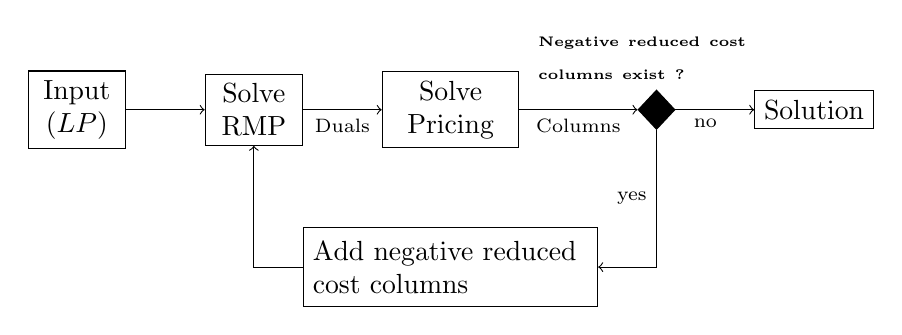
\begin{tikzpicture}
        \node (input) [draw,text width=1cm,align=center] {Input $(LP)$};
        \node (rmp)[text centered,text width = 1cm,draw,anchor=north,right=of input]{Solve RMP};
        \node (pr)[draw,right=of rmp,text centered,text width=1.5cm]{Solve Pricing};
        \node (check) [diamond, right=1.5cm of pr,draw, fill=black, minimum height=0.5cm] {};
        \node (checklab)[above=of check, above=0.0 of check, text width=3cm] {\textbf{\tiny Negative reduced cost columns exist ?}};
        \node (addcol)[draw,below=of pr,minimum height=1cm, text width=3.5cm]{Add negative reduced cost columns};
        \node (solution)[draw, right=of check] {Solution};


        \path[->] (input)    edge (rmp)
                  (rmp)      edge node[below]{\scriptsize Duals} (pr)
                  (pr)       edge node[below]{\scriptsize Columns} (check);
        \draw[->]    (check) |- node[near end, below]{\scriptsize no} (solution);
        \draw[->]    (check) |- node[near start, left]{\scriptsize yes} (addcol);
        \draw[->]    (addcol) -| node[near start,below]{} (rmp);

    \end{tikzpicture}

\end{document}
